\setcounter{chapter}{4} %this gives Chapter 5
\chapter{First observations}
\label{chapter:firstobs}

This chapter describes the preparation of the Sandia trap for operation. Preliminary tests of the \CaI{} oven were conducted. Assembly and bake-out of the vacuum system took place. The \CaI{} oven was tested in experimental conditions by observing neutral atom fluorescence, to characterise the oven and the neutral excitation 423\nm\, laser beam, as a necessary step towards attempts to produce and trap ions.


%\section{Preliminary \CaI{} oven experiment}
\section{Preliminary Ca oven experiment}
\label{sec:oventest}

In the course of preparing the \CaI{} oven for the experiment, suitable electric current parameters had to be estimated. Too high a current would cause \CaI{} deposits on the ion trap chip, while too low a current would not  provide an observable flux of \CaI{}.

David J. Szwer conducted a series of experiments to determine the temperature of a \CaI{} oven as a function of the driving current \cite{Szwer2007}. This calibration can be compared to the records of running other \CaI{} ovens in previous ion traps in our lab.

DJS prepared an oven as described in Section \ref{subsec:oven} (page \pageref{subsec:oven}). It was filled with granules of calcium metal under dry nitrogen to reduce oxidisation. The oven was mounted on stainless steel rods inside a simple vacuum chamber, with thermocouples attached to its surface. 

As current was passed through the oven, the thermocouples measured its temperature. It was found that the thermocouples appeared to underestimate the temperature of the oven. To calibrate the thermocouples, an optical pyrometer (made locally) was used to estimate the temperature of the oven. This operated in the temperature region where the glow of the oven was visible, and it was assumed afterwards that the calibration can be extended from the high temperatures down to room temperature.

Measurements were made up to 9A drive current. The results for oven temperature and oven resistance as functions of driving current are presented in Figure \ref{oventemp}. Earlier ovens were operated at $\sim$300\degC\, \cite{Lucas2004}, which corresponds to 5.5A drive current for the oven described above.


\begin{figure}[t]
\centering
%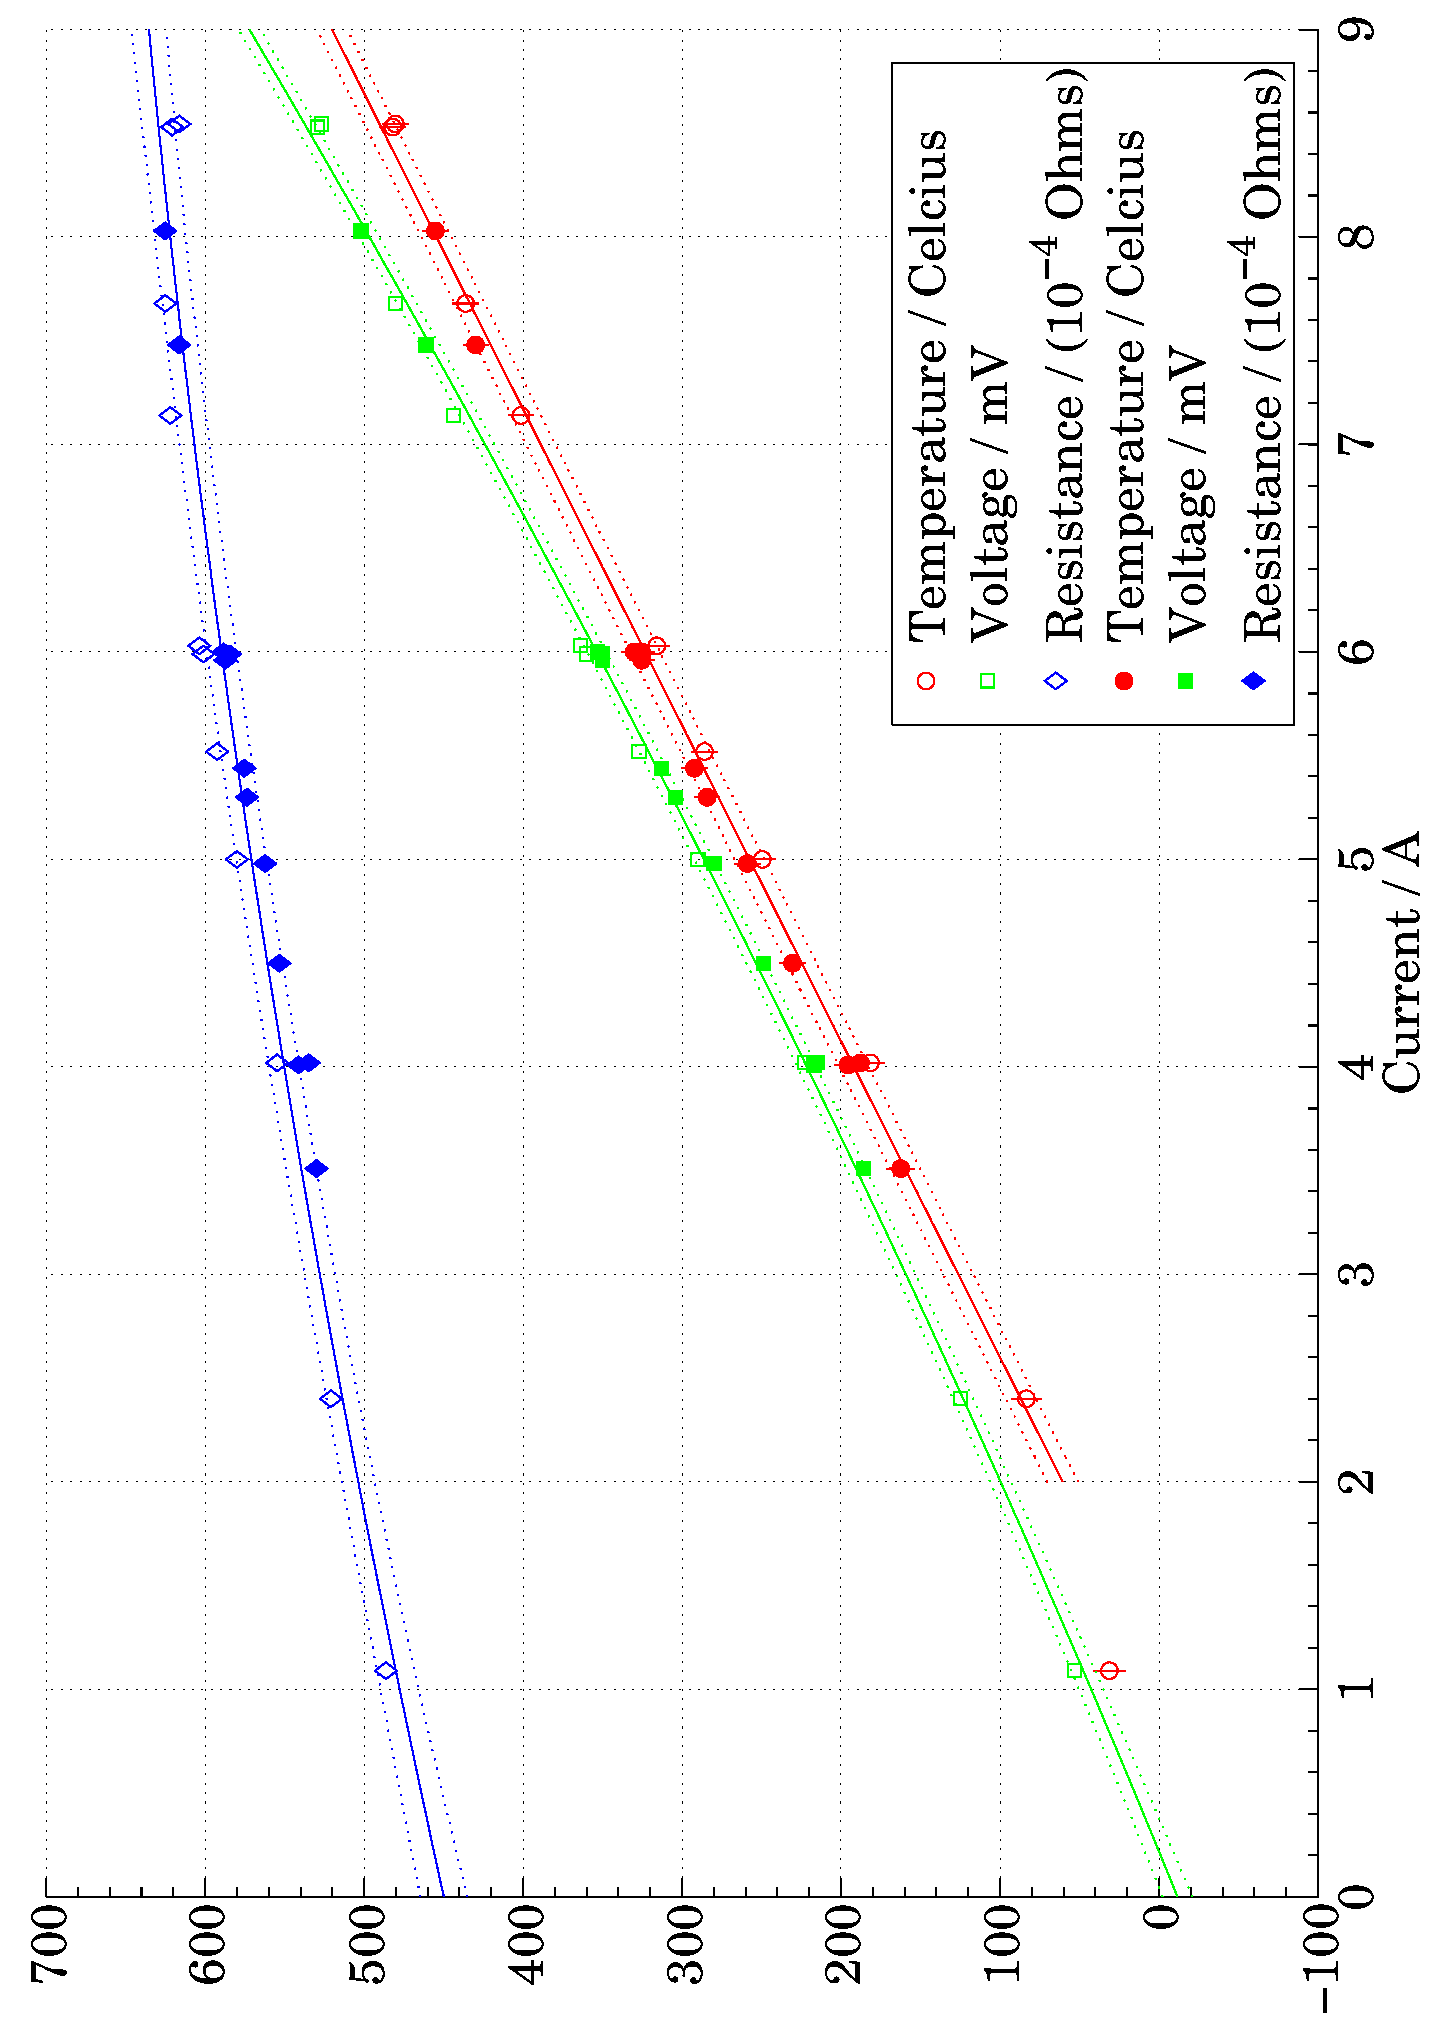
\includegraphics[width=10cm,angle=270]{chapter5/oventest/ovenExptGraph}
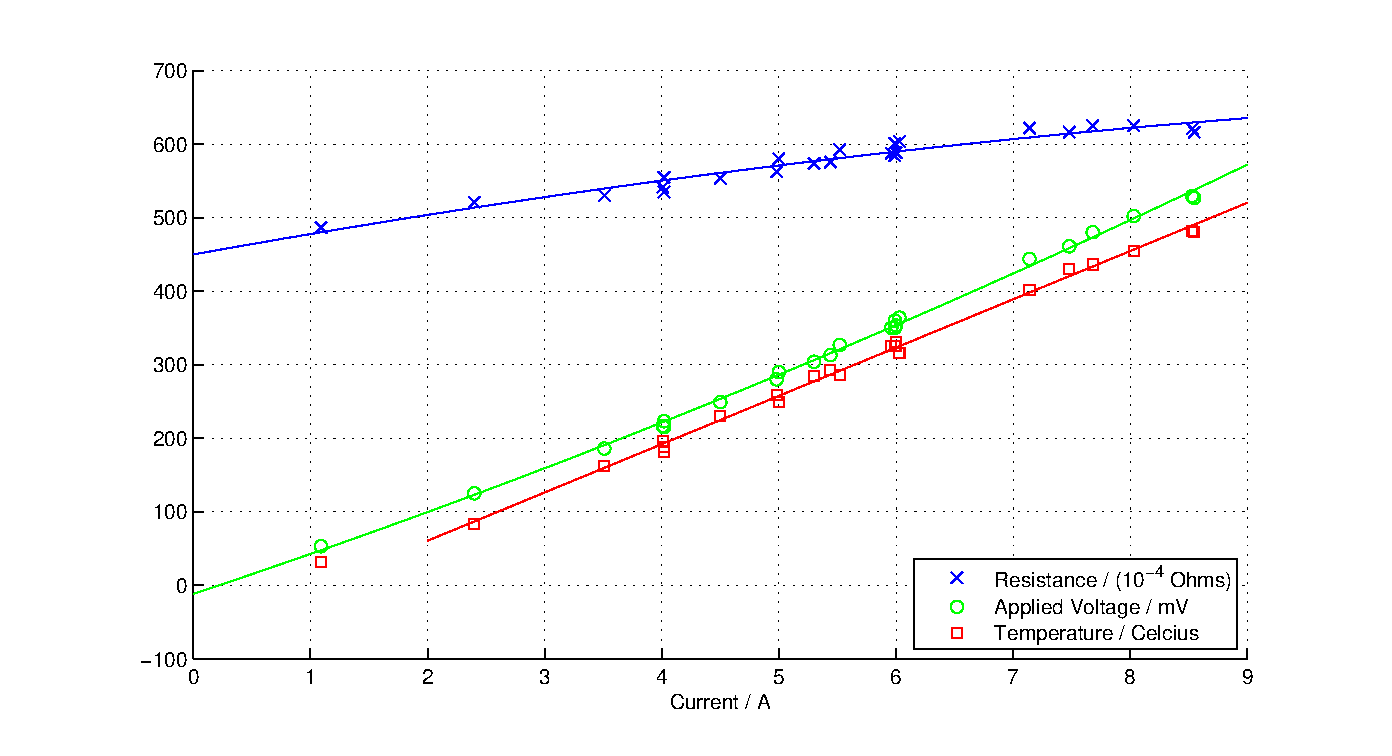
\includegraphics[width=15cm]{chapter5/oventest/oventest_v2}
\caption[Pyrometric oven temperature measurements]{Results of \CaI{} oven test experiment. Temperature, voltage drop and resistance of a \CaI{} oven are shown as functions of applied drive current. The data are combined from two experimental runs. Temperatures are measured by thermocouples and have been corrected with reference to an optical pyrometer, see text. The solid lines are polynomial fits to the data.  (Colour in electronic version.)}
\label{oventemp}
\end{figure} 


\section{Bake-out of the vacuum system}

The assembly and bake-out of the vacuum system took place in several steps. Some experimentation with the bake-out oven was needed to set up the hardware (electronics, heating elements, thermal insulation) and diagnostics logging system.  The elements of the vacuum system had different maximum temperature limits. At different stages of the preparation, as the more temperature-sensitive parts were assembled, the system was baked out at reduced temperatures.  Also, the Sandia ion trap needed structural changes to its RF electrodes, as described in Section \ref{subsec:sandiatrap}, which delayed its installation.

During the bake-out, 8 thermocouples were attached to different parts of the vacuum system, monitoring the temperature to ensure that no part overheated. The temperature measurement was also used to monitor the performance of the heater units, each consisting of  2 1000\W\, RS 196-6464 ceramic heating elements. The voltages supplied to the heater units were limited by variable AC transformers, to reduce the possibility of destructive electronic failures (accidental overheating). The air inside the oven was circulated by a fan, to provide a more uniform temperature.

\begin{figure}[t]
\centering
\includegraphics[width=8cm]{chapter5/bakeout/bakeout}
\caption[Schematics of the bake-out oven]{Schematics of the bake-out oven, with the vacuum system.}
\label{bakeout_oven}
\end{figure} 

\subsubsection{Bake-out} 

The first bake-out took place starting on 11 May 2006. The system consisted of the vacuum chamber and the tubes for connecting the chamber to the ion gauge, the ion pump and the chemical getter pump. The electrical wiring inside the vacuum can, the \CaI{} oven and the ion trap were not installed.

This ``hard bake'' of the vacuum can took 6 days: one day warm up to the maximum 300\degC\, temperature, 4 days at that temperature, and one day to cool down. For the second bake-out, the ion gauge, the ion pump and the chemical getter pump were installed. This bake-out started on 2 Jun 2006. It took 3 days to achieve the maximum temperature of 280\degC. This was maintained for 6 days, after which the system took a further day to cool down. After the bake-out, the magnets of the ion pump were assembled, and the pump's operation was tested.

For the final bake-out, the \CaI{} ovens were installed, the ion trap was mounted in its place inside the vacuum chamber and the ribbon cable connecting a voltage feedthrough and the ion trap DC electrodes was put in place. 

In this bake-out, the maximum temperature was limited by the Kapton insulation of the ribbon cable. Kapton is a polyimide, widely used in industry, and has the advantageous property of very low outgassing rate. However, it is created chemically in temperatures of 200-300 \degC. Because of this manufacturing process, during the bake-out the maximum temperature was limited to $\sim 200\degC$. Higher temperatures could lead to short circuiting and electrical failure of the DC electrodes, which are difficult to repair after the bake-out. The bake-out took 14 days starting on 22 Feb 2007, with a maximum temperature of 200\degC. 

\begin{figure}[t]
\centering
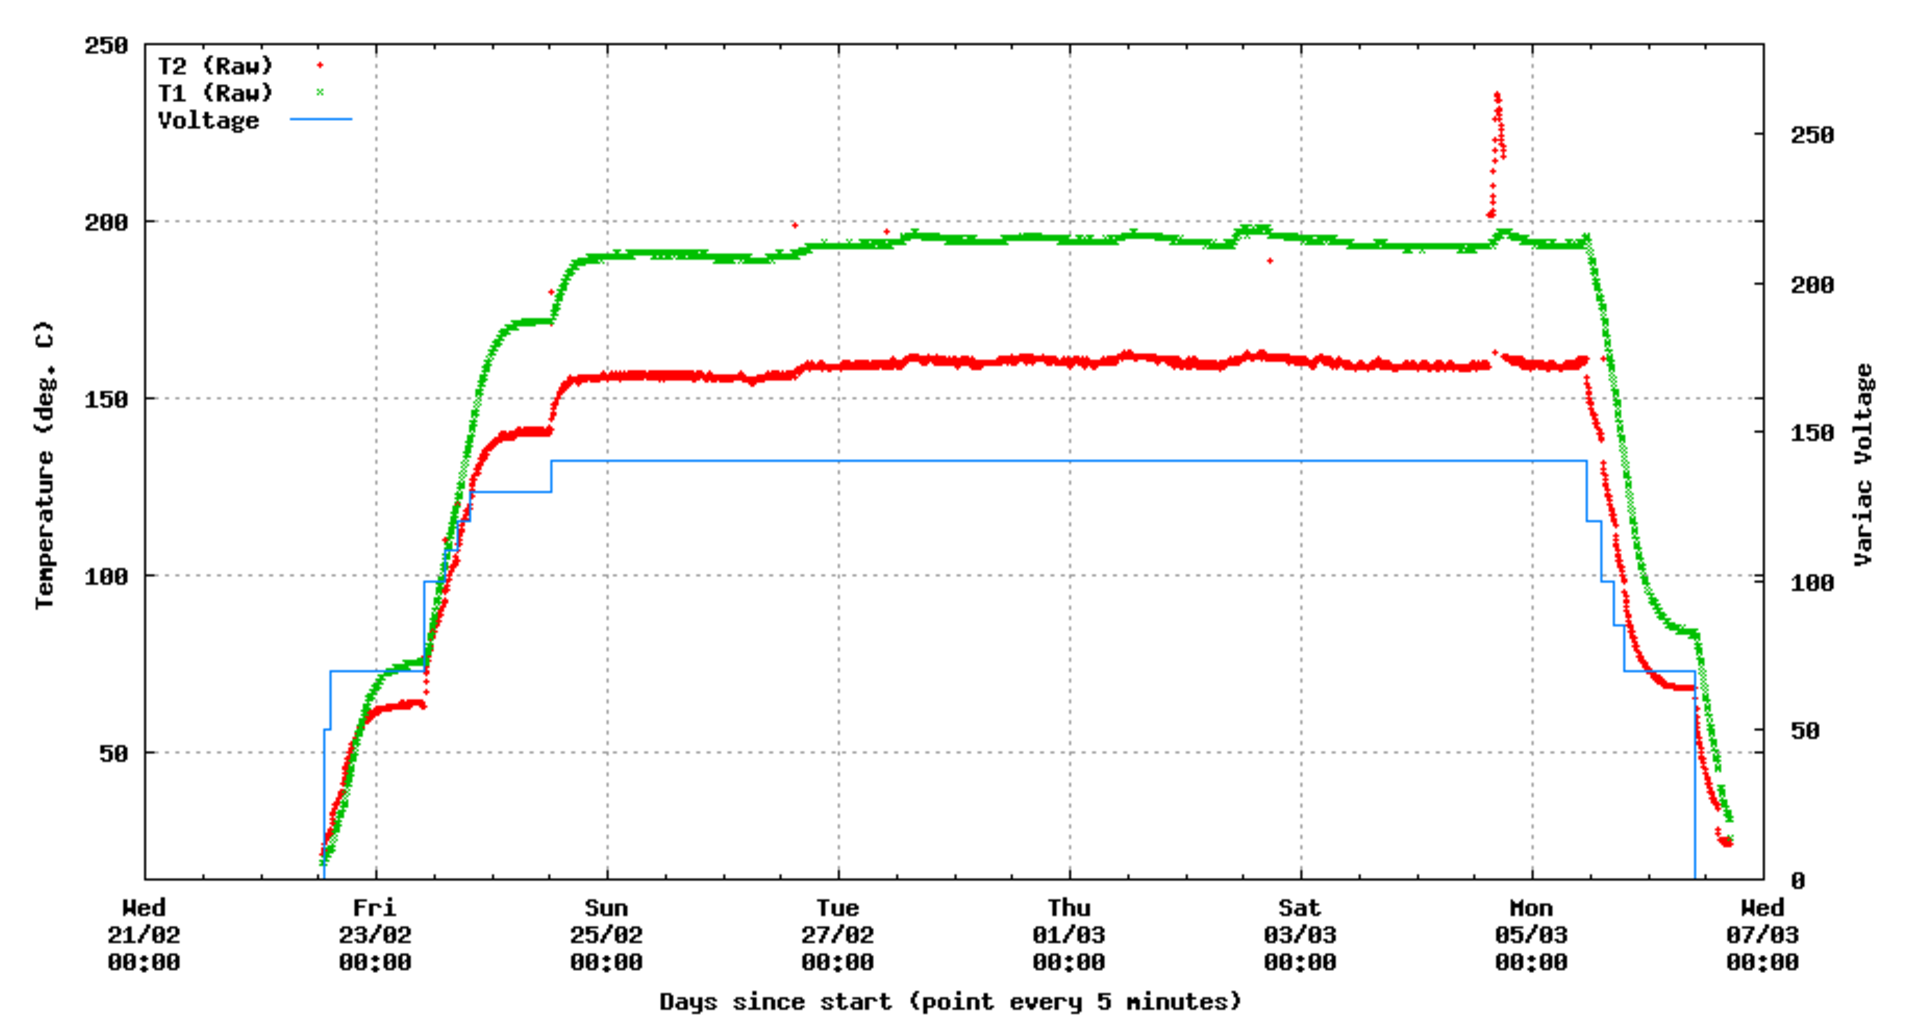
\includegraphics[width=13cm]{chapter5/bakeout/latest-alldays}
\caption[Final bake-out temperature/voltage record]{Temperature vs. time, and heater voltage vs time, during the final bake-out run. T1 and T2 are the temperatures measured by thermocouples taped to the hemisphere, and close to the top of the oven, respectively. Voltage is the drive voltage of the heater units.  \cversion}
\label{bakeout_timerecord}
\end{figure} 

\begin{figure}[t]
\centering
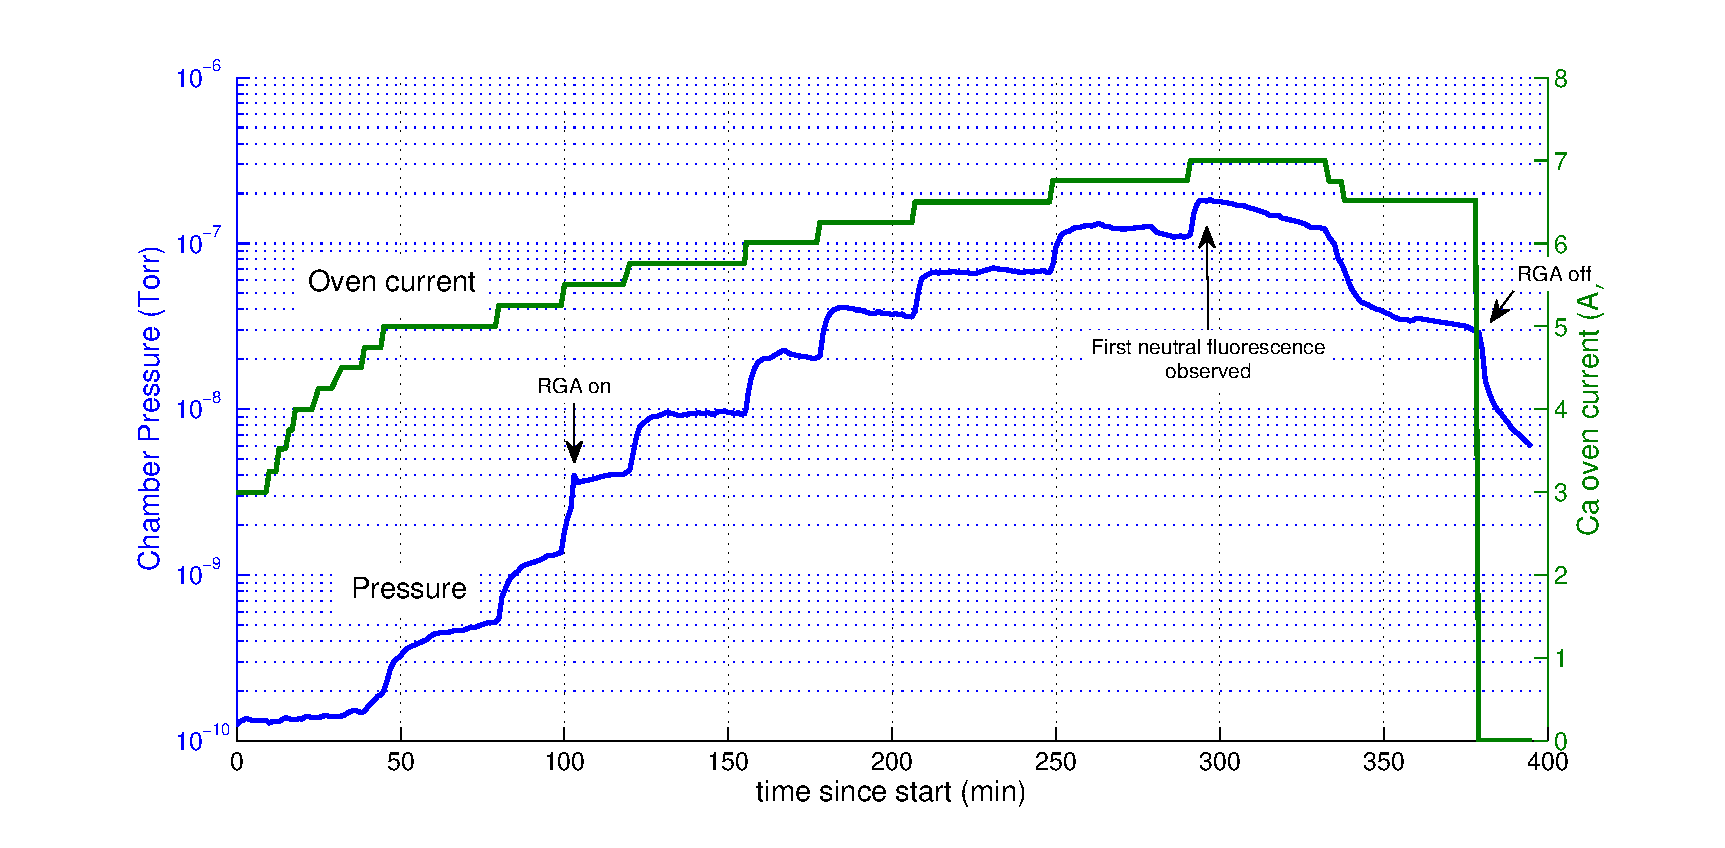
\includegraphics[width=14.2cm]{chapter5/ovenstart/pressure_ovencurrent_3}
\caption[Pressure during \CaI{} oven degassing]{Pressure during the \CaI{} oven degassing. The first observed neutral fluorescence is noted on the plot, at 7A oven current. Turning on the Residual Gas Analyser (RGA) temporarily increased the pressure. Each increase of the oven current resulted in increased pressure. The current was kept at the same level until the pressure approached equilibrium.}
\label{degassing_pressure}
\end{figure} 



\section{Neutral atom fluorescence}
\label{sec:atomfluo}

In the primary bake-out the calcium ovens were degassed only to the same extent as the rest of the vacuum system. The ovens were not heated up to their nominal operating temperature of 300-450\degC\, by driving current through them. Thus inside the metal tube of the oven, absorbed in the calcium, was a supply of gases and a possible oxide layer on the surface of the calcium that had to be cleared out before the oven could operate. 

To carry out a controlled degassing of the oven, the vacuum system was moved to its place in the experimental setup. A 423\nm\, laser beam was focused to the trap centre through the top viewport of the vacuum chamber. During the degassing, scattered light levels from the interaction region were recorded by a PMT while scanning the 423\nm\, laser frequency, checking for neutral \CaI{} fluorescence. In another lab, the same 423\nm\, light was used in a known ion trap,from which the neutral fluorescence was monitored, providing information about the location of the atomic resonance in our frequency scan range. Also, a Residual Gas Analyser (RGA) monitored the gases leaving the oven. Pressures inside the vacuum chamber were recorded. 

The current driving the calcium oven was increased from a starting value of 3\A\, in 0.25\A\, steps, and kept constant until the pressure inside the vacuum chamber was clearly stabilizing. The time-record of the vacuum chamber pressure and oven current is shown in Figure \ref{degassing_pressure}. The first observation of neutral fluorescence was recorded shortly after increasing the oven current to 7\A\, (see Figure~\ref{firstsignal}).



\begin{figure}[t]
\centering
%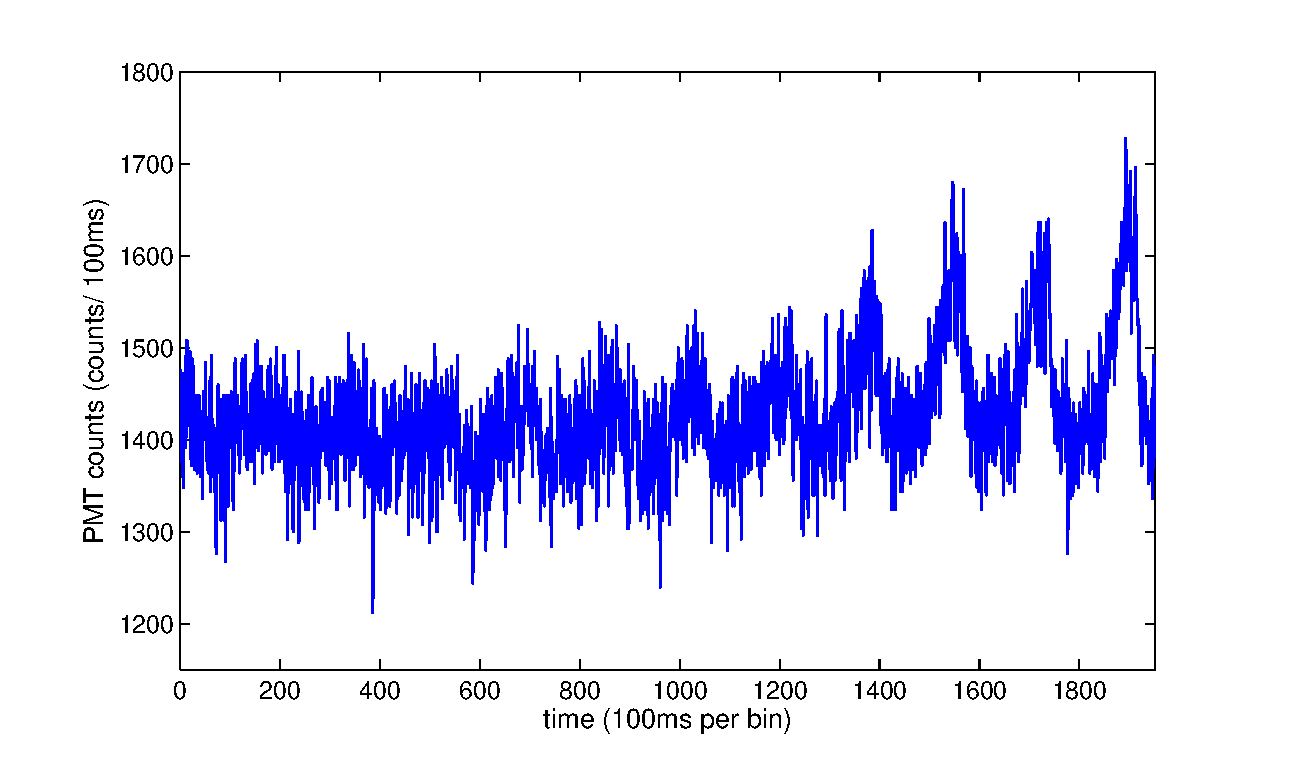
\includegraphics[width=14.2cm]{chapter5/photion/423_firstlight}
%\caption[First observation of neutral fluorescence]{First observation of neutral fluorescence in the Sandia trap. The fluorescence signal is shown as function of time, where the frequency of the 423\nm\, laser was scanned, with a rate of 180bins/scan and 100\ms/bin. The oven current was increased shortly before the above scan was taken (see Figure \ref{degassing_pressure}). The resulting increase in oven temperature is responsible for the growth in the fluorescence signal across the plot.}
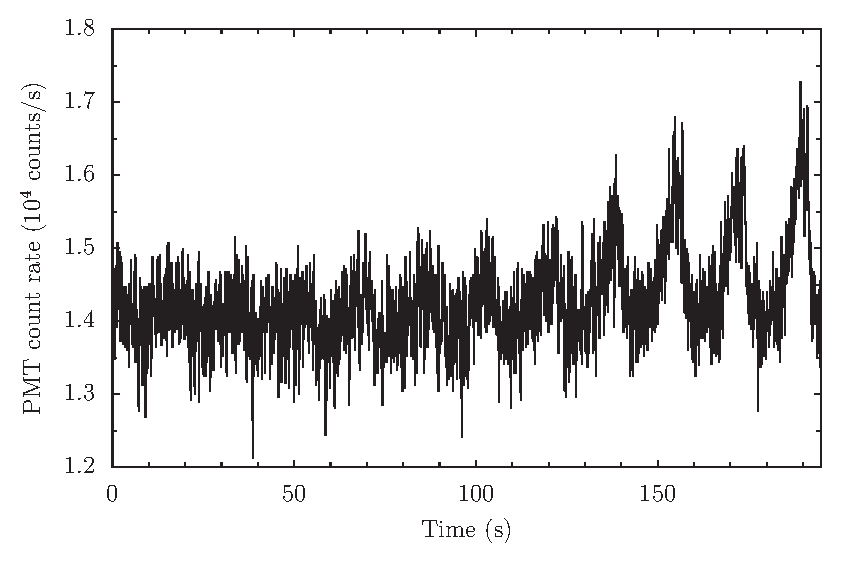
\includegraphics{chapter5/photion/firstlight_v2}
\caption[First observation of neutral fluorescence]{First observation of neutral fluorescence in the Sandia trap. PMT count rate  is shown as function of time, where the frequency of the 423\nm\, laser was repeatedly scanned, with a rate of 18\s/scan. The oven current was increased shortly before the above scan was taken (see Figure~\ref{degassing_pressure}). The resulting increase in oven temperature is causing the growth in the fluorescence signal across the plot.}
\label{firstsignal}
\end{figure} 


%After degassing of the oven, experiments were conducted to characterise the performance of the oven and the $423\nm$ laser beam, in preparation for photoionisation. Fluorescence from the mentioned atoms was recorded as a function of laser frequency, while parameters such as laser intensity and oven currents were changed. The recorded spectra is Doppler-broadened due to the non-perpendicular crossing of the atomic beam and laser beam. In the following section the expected fluorescence spectra is described. This was used to fit the observed fluorescence profiles.

After the first degassing, a pair of experiments were conducted to characterise the 423\nm\, laser beam and the \CaI{} oven. In the first experiment the oven current was held constant, and the intensity of the 423\nm\, beam was varied. In the second experiment the laser intensity was held constant and the oven current was varied. In both experiments, the 423\nm\, frequency was scanned over the atomic resonance and the recorded fluorescence spectrum was fitted with a theoretical profile, which is described in the next section.



% \begin{figure}[h!t]
% \centering
% 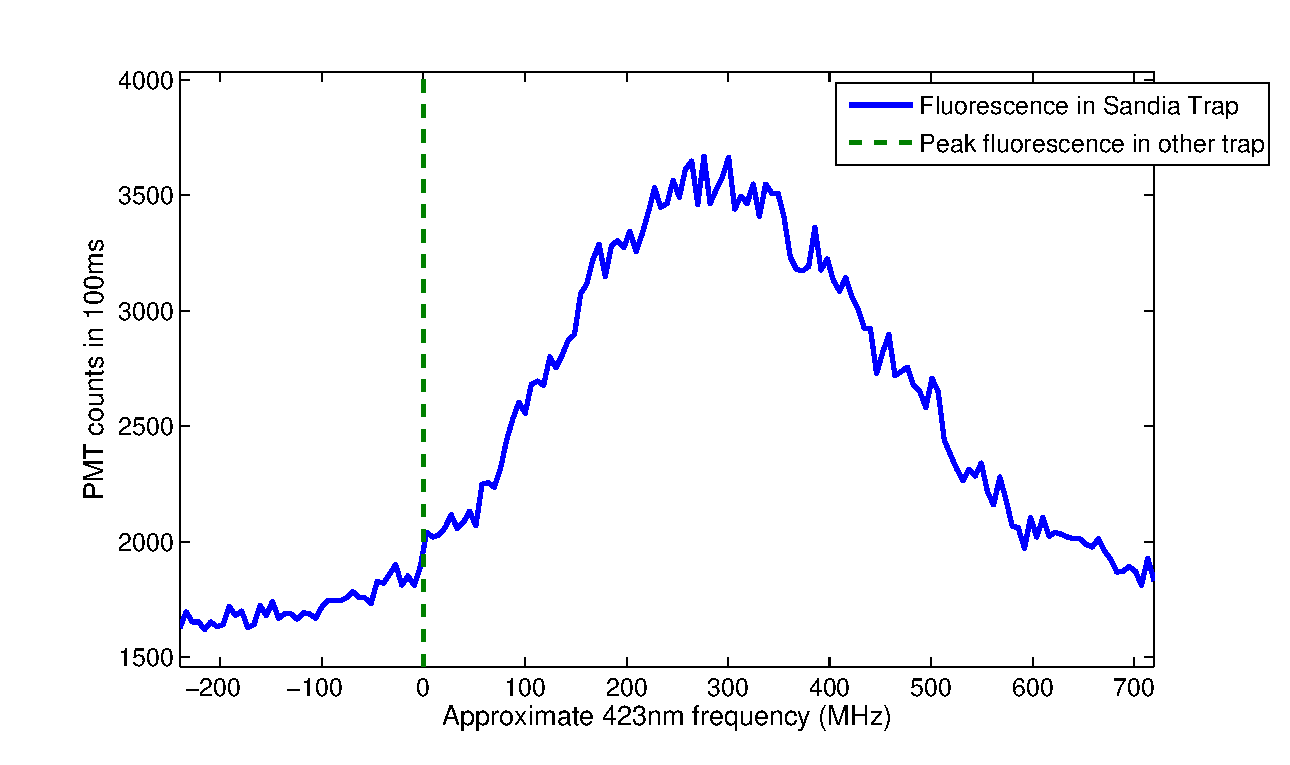
\includegraphics[width=10cm]{chapter5/photion/423_doppler_01}
% \caption[Example distribution]{Example distribution (First? Latter? Fitted?)}
% \label{exampledtibution}
% \end{figure} 

\begin{table}[t]
\begin{center}
\begin{tabular}{|l|c|c|c|}
\hline \textbf{Variable} & \textbf{Symbol}  & \textbf{Initial estimate} & \textbf{Best fit} \\ 
\hline  
Length of interaction region	& $d$					&	$2.30 \times 10^{-4}\m$		&  -  \\
Oven to trap distance		&	$l$					&	$2.2 \times 10^{-2} \m$		& - \\	
Angle of orifice normal to atomic beam & $\gamma$				&	10\degree			& - \\
Angle between atomic and laser beam 	&	$\theta$		&	80\degree			& 76.5(1.5)\degree \\
Polarisation angle to detection system & $\varphi$				&	57\degree			& - \\
Gaussian beam waist		&	$w$					&	21.8\um	& 22(4)\um \\	
Oven temperature (at $I_{\mbox{oven}} = 5.25\A$)	&$T$ 	&	600K				& 640(10)\K \\
Detection efficiency	& $\eta$					&	$1.9 \times 10^{-3}$		& - \\
Oven orifice area		& 	$\sigma$				&	$3 \times 10^{-7}\m^2$		& - \\
\hline 
\end{tabular} 
\caption{Summary of measured parameters used in the calculation. Initial estimates are listed, as well as the best fitted values of those that were allowed to float. Fitted values are shown for the experiment described in Section~\ref{subsec:saturationfluo}.}
\label{tab:neutralfluo}
\end{center}
\end{table}



\subsection{Doppler-broadened neutral fluorescence spectra}

% The following derivation of the expected fluorescence profile is based on \cite{Stacey2007}.

In the fitting procedure, the detected fluorescence signal with known detection efficiency is used to estimate the number $N_e$ of excited atoms in the detection region and thus the number density $n$ of atoms in the detection region. This number density is related to the number density $n_o$ inside the \CaI{} oven, which can be translated into oven temperature $T$ using the vapour pressure formula for \CaI{}. The fluorescence profiles are thus used to characterise the \CaI{} oven, the beam size of the 423\nm\, laser beam and the geometry of the atomic and laser beams. Table~\ref{tab:neutralfluo} summarises the parameters used, and their initial estimates. For parameters estimated from the fluorescence, the best fitted values are listed. 

Consider a neutral \CaI{40} atom subject to 423\nm\, radiation of intensity $I$. The probability of excitation to the 4s4p$^1$P$_1$ state is
\be
p(I,\Delta) = \frac{I A^2 /4}{(2 \pi \Delta)^2 + (A/2)^2 + I A^2 / 2}
\label{exciteprob}
\ee
where $A$ is the Einstein coefficient for the transition, $\Delta$ is the detuning and the intensity $I$ is expressed in units of the saturation intensity $I_S$, defined by
\be
I_S = \frac{4 \pi^2 \hbar c A}{ 3 \lambda^3}.
\label{eq:satintdef}
\ee
In Equation~\ref{exciteprob} the effect of the laser line width is not included. The laser line width is of the order of 4 \MHz\, \cite{Lucas2004}, which is small compared to the Doppler-spread of the spectrum (several hundreds of \MHz). Also, the uncertainties in a number of variables have a larger effect on the fit than the laser line width.


In the case of moving atoms, the detuning is:
\be
\Delta = \Delta_L + \Delta_D
\ee
where $\Delta_L$ is the detuning of the illuminating laser from the line-centre of a stationary atom, and $\Delta_D$ is the Doppler shift:
%\be
%\Delta_D = - \frac{\omega_0 v}{2 \pi c} \cos \theta 
%\ee
\be
\Delta_D = - \frac{v}{\lambda} \cos \theta 
\ee
where $\theta$ is the angle between the laser beam and the direction of propagation of the atomic beam (see Figure \ref{fig:angles}), and $v$ is the atom's velocity. 

\begin{figure}[t]
\centering
\includegraphics[width=10cm]{chapter5/angles_v3}
\caption[Angles of atomic beam, laser beam and detection]{The angles used in the text for the calculation of the expected fluorescence signal.}
\label{fig:angles}
\end{figure} 

The probability distribution of $\Delta_D$ is derived from the longitudinal velocity distribution in a volume for an atomic beam:
\be
f(\Delta_D) \der\Delta_D = 4\sqrt{\frac{\beta^3}{\pi}}\Delta_D^2 \exp\left(-\beta \Delta_D^2\right) \der\Delta_D
\label{probdoppler}
\ee
where
\be
\beta = \frac{M \lambda^2}{2 \kB T \cos^2 \theta} 
\ee
where $M$ is the atomic mass, \kB\, is the Boltzmann factor, and $T$ is the temperature of the oven. In Equation~\ref{probdoppler} $f(\Delta_D)$ is normalised assuming that $\Delta_D < 0$, which is the case in our trap, because $\theta$ is less than 90\degree.

The intensity of the laser beam is assumed to follow a Gaussian profile:
\be
I(r) = I_0 \exp(-2r^2/w^2)
\ee
where $r$ is the distance from the axis of the light beam and $w$ is the spot size in the interaction region.

Consider the number of excited atoms ($N_e$) along a length $d$, lying between $r$ and $r+dr$, with velocity defined by $\Delta_D$:
\be
\der N_e (r,I(r),\Delta) = 2\pi r \, \der r \, d \, n \, p(I(r),\Delta) \, f(\Delta_D) \der\Delta_D
\label{dn}
\ee
where $n$ is the total number density of atoms in the interaction region.

To calculate the number of excited atoms in the interaction region, we have to integrate Equation \ref{dn} over $r$ and $\Delta_D$. To simplify the integral over $r$ we write
\be
\alpha (\Delta_D) = \frac{(2 \pi \Delta)^2 + A^2/4}{I_0 A^2 /2} 
\ee
and
\be
x = 2r^2 / w^2.
\ee
Then
\be
N_e = \frac{\pi n d w^2}{4} \int\int\frac{1}{\alpha(\Delta_D) \exp(x) + 1}dx f(\Delta_D) \der\Delta_D = \frac{\pi n d w^2}{4} C
\label{nequation1}
\ee
where
\be
C = \int \ln \left\{1 + \frac{I_0 A^2/2}{(2 \pi \Delta)^2 + (A/2)^2}\right\}f(\Delta_D) \der\Delta_D .
\ee
We note that in the case of laser intensity  well below saturation ($I_0 \ll 1 $), this expression can be simplified using $\ln(1+x) \approx x$ when  $x \ll 1$:
\be
N_e = \frac{\pi n d w^2 I_0}{4} \int \frac{A^2/2}{\Delta^2 + (A/2)^2}f(\Delta_D) \der\Delta_D 
\label{nequationapprox}
\ee
We obtain the observed count rate $S$ of the fluorescence from the number of excited atoms in the interaction region as
\be
S = \eta N_e A \rho 
\label{signal}
\ee
where $\eta$ is the efficiency of the detection system for isotropically radiated light, and $\rho$ is a factor to take into account polarisation effects in the detection system and the angular distribution of the scattered light. Following a calculation of $\rho$ in \cite{Webster2005}, if the polarisation of the incident light is at angle $\varphi$ to the axis of the imaging system:
\be
\rho = \frac{3}{2} \sin^2 \varphi
\ee
Now we need to relate the number density $n_0$ in the \CaI{} oven to $S$. 
We can obtain the number of excited \CaI{40} atoms in the interaction region as
\be
N_e = \frac{2 S}{3 \eta A \sin^2 \varphi} = \frac{1}{4} \pi n d w^2 C
\label{nsexpress}
\ee
using equation \ref{nequation1}. Hence the number density in the interaction region is
\be
n = \frac{8 S}{3 \pi d w^2 \eta A C \sin^2 \varphi}
\label{numdenssignal}
\ee
This is related to $n_0$ as
\be
n = \frac{n_0 \sigma \cos \gamma}{4 \pi l^2}
\label{eq:n_n0}
\ee
where $\sigma$ is the area of the oven aperture, $l$ is the distance from the oven to the interaction region, and $\gamma$ is the angle between the normal to the aperture and the atomic beam. Thus
\be
n_0 =  \frac{32 l^2 S}{3 d \sigma w^2 \eta A C \cos \gamma \sin^2 \varphi}
\ee
The oven contains other isotopes besides \CaI{40}, so we have to include the relative abundance of \CaI{40} in the expression. In the oven used, this is the natural abundance $a_{40} = 0.969$. The complete number density of \CaI{} in the oven is thus
\be
n_{0,Ca} =  \frac{32 l^2 S}{3 a_{40} d \sigma w^2 \eta A C \cos \gamma \sin^2 \varphi}
\label{numdensoven}
\ee
The number density inside the oven is related to the $p$ vapour pressure of \CaI{} as
\be
n_{0,Ca} = \frac{p}{\kB T}
\label{eq:np}
\ee
The vapour pressure has an experimentally determined dependence on temperature. The empirical formula from the literature \cite{Barin1993} is:
\be
\log_{10}p[\torr] = -52.23 \frac{U}{T [\K]} + B
\label{eq:pt}
\ee
where $p$ is in \torr, and $T$ is in \K. For our temperature region, the constants are $U=195,B=9.697$. By combining Equations~\ref{eq:np} and \ref{eq:pt} we can determine the oven temperature from the number density.


\subsection{Saturation effects}
\label{subsec:saturationfluo}


\begin{figure}[t]
\centering
\includegraphics[angle=0,width=14cm]{chapter5/423layout_v3}
\caption[Layout of the neutral fluorescence experiments]{Layout of the experiment for varying 423\nm\, laser power. Vertical breaks in the laser line indicate additional optical elements for beam guiding.}
\label{fig:423neutralexpt}
\end{figure} 

In the first experiment with neutral \CaI{} atoms the 423\nm\, laser power was varied while the oven current was kept constant. This allowed us to derive the laser beam size and incidence angle, as well as the number density of neutral atoms and oven temperature at the given oven drive current.

The optical setup is outlined in Figure~\ref{fig:423neutralexpt}. The laser beam is coupled into an optical fibre to transfer it to the trap, which ensures that the beam profile stays the same at the output end, regardless of the laser power. The laser power is adjusted by using different neutral density filters on the fibre input end, and measured after the vacuum chamber with a power meter. The laser power and the peak intensity are connected by
\be
I_0 = \frac{2}{\pi w_H w_V}P
\ee
where $w_H$ and $w_V$ are the Gaussian beam spot size in two orthogonal directions (in this case, horizontal and vertical, respectively). When measuring the beam profile, $w_H$ and $w_V$ can be observed separately, while from fitting the data, only the geometric average beam size $w' = \sqrt{w_H w_V}$ can be deduced. The beam parameters were measured with a CCD camera as $ w_H = 19\um $ and $ w_V = 25\um $ ($w' = 21.8\um$), before aligning the beam into the trap.


The observed fluorescence is recorded as a function of the laser frequency, scanning over the Doppler-broadened transition. The signal is fitted as
\be 
S = K_1 C(\Delta,X) + B  \frac{I_0(\Delta)}{I_0(0)}
\label{fulls}
\ee
where B is a fitted parameter associated with the background scatter, 
\be
K_1 = \frac{\pi \eta A \rho n d w^2}{4}
\ee
and
\be
C(\Delta,X) = \int \ln \left\{1 + \frac{I_0(\Delta) A^2/2}{\Delta^2 + (A/2)^2}\right\}f(\Delta_D,X) \der\Delta_D
\ee
and because the oven temperature and the laser incidence angle influence the spectra the same way, they are fitted as a single parameter:
\be 
X = T \cos^2 \theta
\label{tcosth}
\ee
Equation~\ref{fulls} includes the possibility that the laser intensity varies with the laser frequency, expressed as
\be
I_0(\Delta) = \frac{2}{\pi w^2} (P + K_2 \Delta)
\ee
where $P$ is the measured laser power at zero detuning and $K_2$ is a fitted slope parameter. All detunings are expressed as the measured laser frequency and an offset (that has to be fitted):
\be
\Delta = \Delta_{\rm measured} + \Delta_{\rm offset}
\ee

One also has to compensate for the fact that the measured laser power is less than the power experienced by the atoms, due to losses on the exit window and the mirror before the power meter. Because the window does not have an anti-reflection coating for the 423\nm\, wavelength, based on previous experience we assumed a 10\% loss. Thus all measured $P$ laser powers are scaled up by 10\% in the subsequent analysis.


\begin{table}[t]
\begin{center}
\begin{tabular}{|c|c|}
\hline \textbf{Parameter} & \textbf{Fitting type}  \\ 
\hline 
$K_1$ & (global) / individual \\
$K_2$ & individual \\
$X$ & global \\
$B$ & individual \\
$\Delta_{\rm offset}$ & individual \\
$w$ & global \\
\hline 
\end{tabular} 
\caption{The list of fitted parameters of the experiment in Section~\ref{subsec:saturationfluo}. Parameters with ``individual'' fitting had separate value for each scan, while global parameters had a single value for the complete experiment.}
\label{tab:neutralfluofit2}
\end{center}
\end{table}

\begin{figure}[t]
\centering
\includegraphics{chapter5/photion/power2/neutralsatfit_v2}
\caption[Neutral fluorescence signal at different 423\nm\, laser intensities]{Examples of recorded neutral fluorescence as a function of 423\nm\, laser detuning, at different laser intensities (11 scans were taken in total).  The theoretical fit and the residuals are shown. Note the transition in the residuals from statistical variations in a small signal at low power to systematic behaviour due to intensity variations at high power (see text).}
\label{fig:neusatscans}
\end{figure} 


\begin{figure}[h!t]
\centering
\includegraphics{chapter5/photion/power2/neutralsatbg_v2}
\caption[Background scatter of the 423\nm\, beam]{Fitted background counts are shown as a function of measured 423\nm\, laser power. The solid line is a linear fit with zero intercept, with slope of $9.05(6)~\times~10^{3}$counts/\s/\uW.}
\label{fig:background_power}
\end{figure} 

Table~\ref{tab:neutralfluofit2} summarizes the fitted parameters. Due to the setup of the experiment, certain parameters should be the same for all scans: the laser incidence angle $\theta$, the laser beam size parameter $w$ and the number density $n$ of \CaI{} atoms in the interaction region. The incidence angle should be stable because the beam is not moved, the laser beam size because the fibre keeps the beam shape regardles of the input laser power, and the number density because the oven drive current (and thus temperature) is not changed throughout the experiment. However, early in the data analysis it was discovered that it is not possible to reconcile these three global parameters completely because the quality of the scans was insufficient. With such high background, laser intensity variations turned out to be the limiting factor.

In the low intensity scans the residuals were mostly statistical in nature, while the high intensity scans had low signal-to-noise ratio due to high background scatter levels, and the residuals appeared to have a systematic structure, comparable in size to the fluorescence signal (see Figure~\ref{fig:neusatscans}). This made the fits of the high intensity scans less reliable. In general these high frequency intensity variations do not necessarily alter the outcome of the fit, but we note that a slow variation is also present, as shown by the fit parameter $K_2$. There are likely to be also medium frequency variations, that would indeed change the fitted signal height and cannot be factored out.

The high frequency variations are thought to be due to unwanted optical feedback from the fibre input coupler to the laser. The fibre input had a flat-polished face, which does not prevent back reflection. As the laser intensity was adjusted before the fibre coupler, the reflected light had to go through the neutral density filters twice. At low intensities this must have reduced the reflected light to a level which did not affect the laser, but at high intensities it was enough to cause irregularities in the laser output. Using lower laser intensities, replacing the fibre with an angle-polished version, or installing an optical isolator in the beampath before the fibre coupler would provide more stable laser operation. 

The presence of systematic errors due to laser intensity variations prevents a rigorous statistical analysis of the data, so we proceeded as follows. It was possible to fit the recorded spectra with the parameters $w$ and $X$ kept global, while the atomic number density (thus the parameter $K_1$) was floated for all scans. An average value of $n$ could then be found. The best fit parameters under these conditions are
\begin{align}
n & = 8(1) \times 10^{11} \m^{-3} \Longrightarrow T = 640(5) \K \\
X & = T \cos^2 \theta = 35 (3) \K \Longrightarrow  \theta = 76.5(1.5)\degree \\
w & = 22 (4) \um
\end{align}

To assess the reliability of the power measurements, the fitted background scatter is plotted as a function of the measured laser power (see Figure~\ref{fig:background_power}). A linear function with zero intercept fits the data points well, and yields $9.05(6)\times10^{3}$counts/\s/\uW\, as the measure of the background. 



\subsection{Oven temperature as a function of oven current}
\label{subsec:tempovenfluo}

The second experiment is aimed at characterizing the \CaI{} oven. The oven temperature was estimated as a function of the supplied oven drive current. The oven current was adjusted between 5.25\A and 7\A. At a given oven current fluorescence spectra was monitored while scanning the 423\nm\, laser frequency. The laser input power was kept constant low value of $P\approx1\uW$ to avoid optical feedback to the laser, as described previously. The fitted values of $\theta$ and $w$ are used in the data analysis. The observed fluorescence is then a function of the number density and the temperature of the \CaI{} oven.


\begin{figure}[t]
\centering
\includegraphics{chapter5/photion/tempt/c44fit_v1}
\caption[Fluorescence signal showing presence Calcium-44 isotope]{Fluorescence signal showing the presence of \CaI{44}. The oven current was 7\A. The solid line is the fit to the recorded counts, using Equation \ref{fullsiso}.}
\label{fig:ca44}
\end{figure} 


One difference compared to the previous fitting procedure is that we observed hints of a fluorescence peak of the \CaI{44} isotope in the recorded signal when the oven is supplied with high current ($6.5-7 \A$) (see Figure \ref{fig:ca44}). Thus the neutral fluorescence spectra was fitted as a sum of two fluorescence curves, one for  \CaI{40} and one for \CaI{44}, shifted by the isotope shift in the 423\nm\, transition, which is $\Delta_{i,44} = 774 \MHz$. The ratio of the peak heights was fixed at the natural abundance ratio. The abundances of \CaI{40} and \CaI{44} are $a_{40} = 0.969$ and $a_{44} = 0.0209$, respectively.

\begin{eqnarray}
\nonumber S & = & \frac{\pi \eta A \rho n d w^2}{4} \int \ln \left\{1 + \frac{I_0(\Delta) A^2/2}{(2 \pi \Delta)^2 + (A/2)^2}\right\} f(\Delta_D) \der\Delta_D\\ 
\nonumber   &  & + \frac{a_{44}}{a_{40}}\frac{\pi \eta A \rho n d w^2}{4} \int \ln \left\{1 + \frac{I_0(\Delta) A^2/2}{(2 \pi [\Delta-\Delta_{i,44}])^2 + (A/2)^2}\right\}  f(\Delta_D) \der\Delta_D\\
  &  & + B\frac{I_0(\Delta)}{I_0(0)}
\label{fullsiso}
\end{eqnarray}
where $n$ is the number density of the \CaI{40} isotope, and $\Delta$ is the detuning of the 423\nm\, laser from the transition in \CaI{40}. To simplify the fitting procedure, a number of substitutions were made, as in the previous section:
\begin{align}
K_1 & = \frac{\pi \eta A \rho n d w^2}{4}, \\
I_0(\Delta) & = \frac{2}{\pi w^2} (P + K_2 \Delta).
\end{align}



\begin{table}[t!]
\begin{center}
\begin{tabular}{|c|c|}
\hline \textbf{Parameter} & \textbf{Fitting type}  \\ 
\hline 
$K_1$ & individual \\
$K_2$ & individual \\
$X$ & fixed \\
$B$ & individual \\
$\Delta_{\rm offset}$ & individual \\
$w$ & fixed \\
\hline 
\end{tabular} 
\caption{The list of fitted parameters of the experiment determining the \CaI{} oven temperature as a function of oven current.}
\label{tab:neutralfluofit3}
\end{center}
\end{table}

Figure~\ref{fig:temp_current} shows the estimated oven temperature. It appears that the estimated temperature in the previous experiment is lower for the same oven current. Since the two experiments were about one month apart, and the first was conducted immediately after the first outgassing of the \CaI{} oven, it is conceivable that chemical changes happened during that one month use (such as more complete breakdown of the oxide layer on the surface of \CaI{}), that changed the vapour pressure inside the oven and thus the temperature estimate. Also, the oven temperature experiment can be considered more reliable than the one presented in the previous section. This is because of better signal properties due to higher number densities at high temperature (higher signal/background ratio) and the moderate laser intensity (no optical feedback to the laser).

Figure~\ref{fig:pressure_current} shows the recorded pressure in the vacuum chamber as a function of oven current. At low oven currents when there was enough atomic flux to observe a neutral fluorescence signal, the pressure barely rises above the baseline. Based on the experience of other ion trap groups, ion loading in similar traps requires a pressure of less than $10^{-9}\torr$, which is achievable in our system.

The experiments described in this chapter were sufficient to determine the required working parameters for the 423\nm\, laser and \CaI{} oven, to attempt ion loading in the Sandia trap. 


\pagebreak 

\begin{figure}[!t]
\centering
\includegraphics{chapter5/photion/tempt/current_temp_v2}
\caption[\CaI{} oven temperature as a function of drive current]{Estimated oven temperature as function of the oven current. The dashed line is the pyrometric temperature measurement data of a similarly prepared oven, described in Section \ref{sec:oventest} on page \pageref{sec:oventest}. A single point at 6.25\A\, oven current shows the estimate of the experiments described in Section~\ref{subsec:saturationfluo}. \cversion}
\label{fig:temp_current}
\end{figure} 

\begin{figure}[h!t]
\centering
\includegraphics{chapter5/photion/tempt/current_pressure_v3}
\caption[Vacuum chamber pressure as a function of \CaI{} oven current]{Recorded pressure inside the vacuum chamber as a function of the calcium oven current. The dashed line shows the baseline pressure when the \CaI{} is turned off.}
\label{fig:pressure_current}
\end{figure} 
